\documentclass[11pt]{article}

\usepackage[]{acl}

\usepackage{times}
\usepackage{latexsym}
\usepackage[T1]{fontenc}
\usepackage[utf8]{inputenc}
\usepackage{microtype}
\usepackage{inconsolata}
\usepackage{graphicx}
\usepackage{booktabs}
\usepackage{multirow}
\usepackage{tabularx}
\usepackage{array}
\usepackage{amsmath}
\usepackage{amsfonts}
\hypersetup{colorlinks=true, urlcolor=blue, linkcolor=black, citecolor=black}
\usepackage{caption}
\usepackage{subcaption}
\usepackage{tikz}
\usepackage{float}
\usepackage{stfloats}
\renewcommand{\topfraction}{0.9}
\renewcommand{\bottomfraction}{0.9}
\renewcommand{\textfraction}{0.05}
\renewcommand{\floatpagefraction}{0.7}
\setcounter{topnumber}{3}
\setcounter{bottomnumber}{3}
\setcounter{totalnumber}{5}
\usetikzlibrary{shapes.geometric, arrows.meta, positioning, fit, backgrounds}


\newcolumntype{C}[1]{>{\centering\arraybackslash}p{#1}}

\title{Structured Extraction of PICO Information from Clinical Trial Abstracts:
A Comparative Study of Rule-Based, Prompted and Fine-Tuned Approaches}

\author{
\begin{tabular}{ccc}
Saisha Hiray & Disen Zhu & Chris Luckhurst \\
\texttt{2822967} & \texttt{2560315} & \texttt{2832364} \\[4pt]
Sanya Kapoor & Han Zongjin & Weixuan Gu \\
\texttt{2696783} & \texttt{2764620} & \texttt{2816084} \\
\end{tabular} \\[8pt]
\textit{Group 2 Introduction to AI and Text Analytics Coursework} \\[2pt]
\small Github link: \url{https://github.com/Blacknomizi/IATA-Coursework-Group2}
}

\begin{document}
\maketitle




\begin{abstract}
Converting clinical trial abstracts to structured tables based on the PICO format has been one of the most important ways to enable large-scale evidence synthesis. Using the EBM-NLP corpus\citep{nye2018ebmnlp}, we compare nine extraction systems along two design
axes namely rule-based versus LLM-based, and end-to-end versus decomposed, on
a locked 50-document evaluation set, and report token-overlap F1, strict span
F1, coverage and downstream keyword query usability. Fine-tuned transformer
models clearly dominate: end-to-end BioBERT achieves a macro
token-overlap F1 of 0.673, narrowly ahead of fine-tuned DistilBERT (0.647)
and well above any prompted LLM (best 0.347 for zero-shot flan-T5). Three
findings emerge as more interesting than the headline ranking. Firstly,
zero-shot beats few-shot for prompted flan-T5 because few-shot instants leak
study-specific phrases (\textit{Rhinocort Study Group}) as learned priors.
Secondly, the value of decomposing extraction depends on the underlying model:
it helps weak QA-based extractors ($+$0.12 macro F1) but hurts strong
supervised ones ($-$0.07 strict span F1) because the relevance filter
over-discards. Third, high coverage does not imply usability, prompted
LLMs return some text for 100\% of documents but retrieve only 1 of 11
placebo-controlled trials in downstream queries, while every fine-tuned and
rule-based system finds $\geq$11.
\end{abstract}


\section{Introduction}

Systematic reviews and meta analyses underpin evidence-based medicine, but a
practising clinician evaluating a treatment must screen thousands of trial
abstracts before identifying a few dozen suitable studies. The PICO schema: \textit{Population}, \textit{Intervention}, \textit{Comparator},
\textit{Outcome} is the standard way of describing a trial in
structured form for retrieval and synthesis \citep{higgins2019cochrane}.
Automated PICO extraction would convert free text abstracts into a queryable
table, allowing reviewers to filter trials by population, group trials with
shared interventions or compute effect sizes across studies that report
comparable outcomes.

We work with EBM-NLP \citep{nye2018ebmnlp}, a corpus of 4{,}993 abstracts
annotated for participants (P), interventions (I) and outcomes (O) at token
level. The dataset combines crowd-worker annotations
(\textit{starting\_spans}, used in the rule-based pipeline of 02\_rule\_based\_vs\_llm.ipynb) with expert-aggregated hierarchical labels
(\textit{aggregated/hierarchical\_labels}, used by every supervised model).
Comparators are folded into the Interventions field by design
\citep[\S2]{nye2018ebmnlp}; we extract only P, I, O, and discuss the
comparator (the ``C'' in PICO) as a dataset level limitation in
\S\ref{sec:limitations}.

\paragraph{Requirements for a good system.} A reviewer using the extracted
table cares about three things, in order of decreasing severity. Recall
matters most because a missed trial is silently dropped from a meta-analysis
and cannot be recovered downstream. Coverage matters next because a row
with empty PICO cells is unusable regardless of the precision of its
populated fields. Precision matters last because false positives can be
filtered manually but false negatives cannot. F1 alone hides the
recall--coverage trade-off, so we report all three throughout this paper.

\paragraph{Example.} A typical abstract from the corpus illustrates what
extraction must recover. PMID 10070173 begins: \textit{``Comparison of
budesonide Turbuhaler with budesonide aqua in the treatment of seasonal
allergic rhinitis. Two hundred and eighty-four out-patients\dots''}. The
gold annotations mark \texttt{seasonal allergic rhinitis} and
\texttt{Two hundred and eighty-four out-patients} as Participants,
\texttt{budesonide Turbuhaler} and \texttt{budesonide aqua} as
Interventions, and \texttt{quality of life} and \texttt{Mean daily nasal
symptom scores} (later in the abstract) as Outcomes. A correct system
must therefore handle multi-span, multi-sentence extraction with both
numerical and noun-phrase entities; cohort sizes and condition
descriptors both qualify as Participants under the EBM-NLP scheme.

\paragraph{Data exploration} Before designing extractors we asked whether
sentence-level structure already separates the schema fields. We embedded
all training sentences with MiniLM \citep{reimers2019sentencebert},
clustered them with $k$-means and HAC at $k\!=\!2 \ldots 8$, and computed
adjusted Rand index, normalised mutual information and silhouette against
gold sentence-level labels (Figure~\ref{fig:silhouette}). The result is
a clear negative: ARI $= 0.012$ and NMI $= 0.007$ against gold for joint
PIO at $k\!=\!3$  essentially indistinguishable from random and
silhouette is roughly flat across all $k$. Sentence embeddings do not
naturally recover the schema, which motivates supervised extraction
(\S\ref{sec:methods}) rather than an unsupervised pipeline. A biomedical
encoder (PubMedBERT-MS-MARCO \citep{deka2022pubmed}) yields a small but
consistent $+$0.018 ARI on the same data, supporting the use of
domain pretrained encoders for downstream extraction without changing
the headline conclusion.


\begin{figure}[tbp]
  \centering
  
\includegraphics[width=\columnwidth]{figures/clustering_silhouette.png}
  \caption{Silhouette score across $k$ for $k$-means on joint-PIO sentence
  embeddings (MiniLM, 3{,}000 sentences). Silhouette declines monotonically
  from $k\!=\!2$ to $k\!=\!8$ with no meaningful peak at $k\!=\!3$, and
  ARI and NMI against gold sentence-level labels are 0.012 and 0.007 
  essentially random. This null result motivates supervised extraction
  (\S\ref{sec:methods}).}
  \label{fig:silhouette}
\end{figure}

\paragraph{Contributions} We have compare nine extraction systems along two
explicit design axes (rule-based vs LLM; end-to-end vs decomposed) on an
identical 50 document locked evaluation set; we share data loading,
prediction storage and evaluation through (\texttt{src/}) so all numbers in this report are computed under the same metric, with the same gold spans, on the same documents.
\textit{Note: NBO* in the entire report refers to respective ipynb file in notebook folder on github}


\section{Methods}
\label{sec:methods}

\subsection{Shared infrastructure and preprocessing}

Every system in this study reads from the same loader, writes predictions
to a JSON file in \texttt{predictions/}, and is graded by the same
evaluator on the same 50 documents. The locked evaluation set is the first
fifty document IDs in the intersection
$\textsc{Test}_P \cap \textsc{Test}_I \cap \textsc{Test}_O$, sorted, and
saved to \texttt{eval\_doc\_ids.json}; reusing this list across notebooks
guarantees comparability when individual notebooks are re-run in
isolation. Hierarchical EBM-NLP labels (0--7) are flattened to BIO tags by
\texttt{hierarchical\_to\_bio}, while the rule-based pipeline uses the
simpler \texttt{starting\_spans} layer because regex patterns operate on
token sequences rather than typed entities.
\paragraph{BIO tag scheme.} For each PICO field $t \in \{P, I, O\}$
independently, a token sequence $\mathbf{x} = (x_1, \dots, x_n)$ receives
binary BIO tags $y_i \in \{B, I, O\}$. Hierarchical EBM-NLP labels
($r_i \in \{0, \dots, 7\}$) collapse to BIO via:
\begin{equation}
y_i = \begin{cases}
O & \text{if } r_i = 0 \\
B & \text{if } r_i \neq 0 \text{ and } r_{i-1} = 0 \\
I & \text{if } r_i \neq 0 \text{ and } r_{i-1} \neq 0
\end{cases}
\label{eq:bio}
\end{equation}
The per field decomposed pipelines (NB04 DistilBERT, NB05 QA, NB06
decomposed BioBERT) train one binary tagger per field. The end-to-end
BioBERT (NB06) instead uses a merged 7-tag schema
($O, B\text{-}P, I\text{-}P, B\text{-}I, I\text{-}I, B\text{-}O, I\text{-}O$)
so a single model emits all three field assignments jointly.(Here all the NB0* refers to respective notebooks (ipynb) from github repo in notebook folder)

We adopt two evaluation metrics. Token-overlap F1 (lenient,
bag-of-tokens) is used to compare all nine approaches, because not all of
them emit BIO sequences. Strict span F1 (exact start/end/type match) is
used inside the supervised notebook to compare end-to-end versus
decomposed under a stricter rule (\S\ref{sec:metrics}). Coverage is the
fraction of documents with at least one non-empty extraction; downstream
usability is measured by four keyword queries against the table
(\S\ref{sec:results}).
\subsection{Pipeline architectures}
\label{sec:architectures}

Figure~\ref{fig:pipelines} shows the four pipeline architectures
implemented in this study. All 4 read the same EBM-NLP abstract
tokens and emit a per field span list, but differ in how they map
between the two: rule-based pipelines uses deterministic pattern
matching, prompted LLMs treat extraction as text generation, end-to-end
transformers tag every token with a joint BIO label, and decomposed
transformers split the work into a sentence-relevance filter and a
per-field tagger.

\begin{figure*}[tbp]
\centering
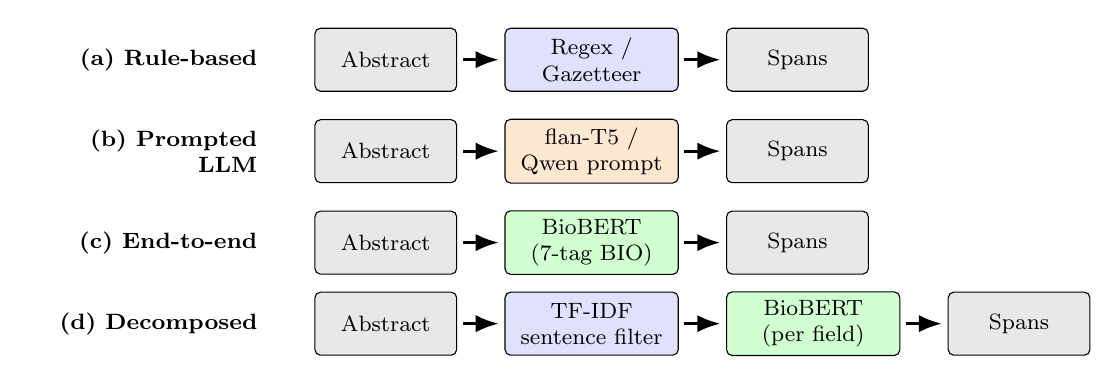
\begin{tikzpicture}[
  font=\footnotesize,
  >=Latex,
  node distance=4mm and 6mm,
  every node/.style={align=center},
  io/.style={draw, rounded corners=2pt, fill=gray!18,
             minimum height=8mm, minimum width=18mm,
             inner sep=3pt},
  proc/.style={draw, rounded corners=2pt, fill=blue!12,
               minimum height=8mm, minimum width=22mm,
               inner sep=3pt},
  llm/.style={draw, rounded corners=2pt, fill=orange!18,
              minimum height=8mm, minimum width=22mm,
              inner sep=3pt},
  bert/.style={draw, rounded corners=2pt, fill=green!18,
               minimum height=8mm, minimum width=22mm,
               inner sep=3pt},
  arr/.style={->, very thick, shorten >=2pt, shorten <=2pt},
  rowlbl/.style={font=\footnotesize\bfseries, anchor=east, text width=28mm,
                 align=right}
]


\node[rowlbl] (la) at (0, 0) {(a) Rule-based};
\node[io, right=6mm of la] (a1) {Abstract};
\node[proc, right=of a1] (a2) {Regex /\\Gazetteer};
\node[io, right=of a2] (a3) {Spans};
\draw[arr] (a1) -- (a2);
\draw[arr] (a2) -- (a3);


\node[rowlbl, below=5mm of la] (lb) {(b) Prompted LLM};
\node[io, right=6mm of lb] (b1) {Abstract};
\node[llm, right=of b1] (b2) {flan-T5 /\\Qwen prompt};
\node[io, right=of b2] (b3) {Spans};
\draw[arr] (b1) -- (b2);
\draw[arr] (b2) -- (b3);


\node[rowlbl, below=5mm of lb] (lc) {(c) End-to-end};
\node[io, right=6mm of lc] (c1) {Abstract};
\node[bert, right=of c1] (c2) {BioBERT\\(7-tag BIO)};
\node[io, right=of c2] (c3) {Spans};
\draw[arr] (c1) -- (c2);
\draw[arr] (c2) -- (c3);

\node[rowlbl, below=5mm of lc] (ld) {(d) Decomposed};
\node[io, right=6mm of ld] (d1) {Abstract};
\node[proc, right=of d1] (d2) {TF-IDF\\sentence filter};
\node[bert, right=of d2] (d3) {BioBERT\\(per field)};
\node[io, right=of d3] (d4) {Spans};
\draw[arr] (d1) -- (d2);
\draw[arr] (d2) -- (d3);
\draw[arr] (d3) -- (d4);

\end{tikzpicture}
\caption{The four pipeline architectures compared are sharing
common input (\textit{Abstract}) and output (\textit{Spans}) but differing
in the intermediate processing.
(a) Rule-based extractors apply hand-crafted patterns or a frequency
gazetteer directly to the tokenised abstract.
(b) Prompted LLMs wrap the abstract in a question prompt and parse
generated text.
(c) End-to-end transformers (BioBERT) tag every token with a single
7-tag BIO label.
(d) Decomposed transformers first filter sentences with a TF-IDF
classifier, then run a per-field BioBERT tagger only on accepted
sentences.}
\label{fig:pipelines}
\end{figure*}

\subsection{Design axis A: rule-based vs LLM}

The first axis asks how much of the task can be solved by symbolic
patterns over the abstract, and how much requires a learned model. We
implement four extractors that span this axis from purely hand-crafted
to fully learned. The simplest is a regex-based extractor (NB02) using
hand-written patterns for cohort sizes
(\verb!\d+\s+(patients|men|women)!), drug doses (\verb!\d+\s*mg!), and
outcome cues such as \verb!side effects! and \verb!score!. One step up
in data-drivenness is the gazetteer (NB02), which extracts the
top-200 1- to 3-grams per field by frequency in 300 training-set gold
spans and matches them at test time as whole-word case-insensitive
regex; this asks how far one can get by simply memorising training-time
spans. We then introduce a small fine-tuned LLM, Qwen3-0.6B (NB02), an
instruction-tuned decoder \citep{qwen2024} given three in-context
examples per field and asked to copy the answer. Finally, three prompt
variants on flan-T5-base \citep[250M parameters,][]{chung2022flan} (NB03)
let us isolate the effect of the prompt itself: zero-shot
question-answering, three-shot worked examples, and three-shot with a
JSON output constraint. All flan-T5 generations use beam search
($n\!=\!4$), 512-token input, and 80--120 output tokens.

\subsection{Design axis B: end-to-end vs decomposed}

The second axis asks whether a single model should emit all three field
assignments at once, or whether the task should be broken into
\textit{find the relevant sentence}, then \textit{extract the span}.
Five systems span this axis. The CRF baseline (NB06) is a linear-chain
CRF \citep{lafferty2001crf} with shape, prefix/suffix and
medical-keyword features; we train one tagger per field and merge
predictions with a P$<$I$<$O priority rule. It is the classical
baseline against which deep models are usually judged. Fine-tuned
DistilBERT (04\_transformer\_finetuned.ipynb) takes the same per-field decomposition into the
deep-learning regime: three independent DistilBERT-base-uncased
\citep{sanh2019distilbert} token classifiers (one per field) trained on
hierarchical NER tags (\texttt{B-1\dots I-4} per field) for 5 epochs at
batch 16, learning rate $1\!\times\!10^{-5}$ and weight decay 0.01.

The end-to-end BioBERT (06\_end\_to\_end\_vs\_decomposed.ipynb) does the opposite: a single
BioBERT-base-cased \citep{lee2020biobert} fine-tuned on a merged 7-tag
schema (O, B-P/I/O, I-P/I/O), with two-phase training that first trains
the classification head for 4 epochs with the encoder frozen, then
fine-tunes the full model for 2 epochs at $2\!\times\!10^{-5}$. The
decomposed BioBERT (06\_end\_to\_end\_vs\_decomposed.ipynb) tests whether the per-field decomposition of 04\_transformer\_finetuned.ipynb also helps when the underlying model has already seen biomedical
text: a TF-IDF + logistic-regression classifier first predicts whether
each sentence contains an entity of a given type, then a per-field
BioBERT token tagger runs only on accepted sentences. Finally,
extractive QA (NB05) uses \texttt{deepset/roberta-base-squad2}
\citep{liu2019roberta} in three configurations end-to-end (one
question per field on the whole abstract), 2-step decomposed (sentence
classification by argmax confidence, then extraction), and 3-step
decomposed (2-step plus post-hoc cleaning: deduplication, $\geq$2-token
spans, and a ``person word'' filter for participants).

\subsection{Hypotheses}
\label{sec:hypotheses}

We motivate the comparison with five testable claims. \textbf{H1}:
LLM-based extractors will beat rule-based extractors, because the latter
cannot generalise beyond the patterns the author thought of.
\textbf{H2}: Few-shot prompting will beat zero-shot, because in-context
examples ground the output format and demonstrate what the answer
should look like. \textbf{H3}: Fine-tuned models will beat prompted
models, because EBM-NLP supplies $\sim$4{,}500 training documents ---
well above the scale at which supervised fine-tuning typically dominates
few-shot prompting. \textbf{H4}: Decomposing extraction into
\textit{filter-then-extract} will improve precision, because background
and methods sentences that contain no PICO entities are eliminated
up-front. \textbf{H5}: BioBERT will beat DistilBERT on this corpus,
because domain pre-training matches the lexical distribution of
biomedical abstracts. Section~\ref{sec:results} shows that H1, H3 and
H5 hold strongly; H2 fails (zero-shot wins); H4 holds only conditionally
on the underlying model.

\subsection{Notes on shortcomings of this design}

The QA approaches (05\_decomposed\_qa\_roberta.ipynb) target axis B alongside NB06's decomposed
BioBERT pipeline, but their saved predictions were generated against a
development-stage document subset before the locked evaluation set was
finalised in \texttt{src/data.py}. NB07(notebook 07 for final comparison in notebook folder on git) detects this automatically: any
approach with zero coverage on the locked set is flagged and excluded
from the master ranking, preventing misleading near-zero F1 values from
polluting Table~\ref{tab:master}. The QA approaches' internal evaluation
in NB05 (macro F1 0.27 end-to-end, 0.39 2-step decomposed, 0.34 3-step)
is reported in Table~\ref{tab:nb05_nb06} so the decomposed-vs-end-to-end
axis remains directly comparable; the underlying QA models are
functional, only the doc-ID alignment is stale. NB06's
relevance-classifier + per-field BioBERT pipeline represents the
decomposed extraction axis in the master ranking.
\textbf{Note}: NB0* refers to respective ipynb file in notebook folder on github

\section{Experimental evaluation}
\label{sec:results}

\subsection{Metrics and their limitations}
\label{sec:metrics}

\paragraph{Token-overlap F1.} Treats predictions and gold spans as token
sets; $P\!=\!|G \cap \hat{Y}| / |\hat{Y}|$, $R\!=\!|G \cap \hat{Y}| /
|G|$. We follow the convention that both empty $\rightarrow$ (1, 1, 1),
gold empty and pred non-empty $\rightarrow$ (0, 1, 0). It is the only
definition that applies uniformly across all nine approaches because
not all of them emit BIO sequences. \textit{Limitation:} a model
returning the single token \texttt{patients} gets partial credit for
the gold span ``Two hundred and eighty-four out-patients with seasonal
allergic rhinitis''. We adopt token-overlap F1 as the report's
\textbf{primary metric} because it applies uniformly across all nine
approaches; strict span F1 is reported in Table~\ref{tab:nb05_nb06} as
a stricter secondary check on axis B, where BIO output is available.

\paragraph{Strict span F1.} Span match requires identical $(\text{start},
\text{end}, \text{type})$ in BIO sequences the standard NER metric.
Used inside NB06 (CRF, end-to-end BioBERT, decomposed BioBERT) where
BIO output is available. \textit{Limitation:} fully penalises minor
boundary errors, so a 1-token shift on a 10-token span scores zero.

\paragraph{Coverage.} Fraction of documents with at least one non-empty
field. A model with high F1 but low coverage is delivering empty rows.

\paragraph{Downstream usability.} For each of four keyword queries
(\textit{trials with placebo}, \textit{trials mentioning patients},
\textit{trials measuring pain}, \textit{trials with rehabilitation}) we
count how many of the 50 extracted PICO rows match the query and
compare against the gold count. This is the only metric that is
end-user-aligned.

\subsection{Setup}

All notebooks read EBM-NLP via the shared loader. Training uses the full
training split per field (4{,}454-4{,}993 docs). Validation for the
transformer models is a 10\% slice of train; the test split is unused
during training. Hyperparameters were chosen to match standard
fine-tuning recipes (E2E BioBERT: warm-up by training the head only at
$5\!\times\!10^{-5}$ before unfreezing at $2\!\times\!10^{-5}$). All
runtimes are reported on Google Colab T4 GPU. Predictions for every
approach are saved as JSON and aggregated by NB07; this means re-running
NB07 alone reproduces every number in Table~\ref{tab:master}.

\subsection{Master comparison: token-overlap F1}
\label{sec:master_comparison}

Table~\ref{tab:master} reports per-approach, per-field token-overlap
P/R/F1 and coverage on the 50-document locked evaluation set, ordered
by macro F1. Figure~\ref{fig:master_f1} shows the same numbers as a
grouped bar chart.

\begin{table*}[tbp]
\centering
\small
\begin{tabular}{l ccc ccc ccc c}
\toprule
& \multicolumn{3}{c}{\textbf{Participants}} & \multicolumn{3}{c}{\textbf{Interventions}} & \multicolumn{3}{c}{\textbf{Outcomes}} & \\
\cmidrule(lr){2-4}\cmidrule(lr){5-7}\cmidrule(lr){8-10}
\textbf{Approach} & P & R & F1 & P & R & F1 & P & R & F1 & \textbf{Macro F1} \\
\midrule
E2E BioBERT          & .874 & .400 & .512 & .727 & .912 & \textbf{.778} & .792 & .727 & \textbf{.730} & \textbf{.673} \\
DistilBERT           & .855 & .382 & .497 & .648 & .842 & .691 & .804 & .748 & .754 & .647 \\
CRF                  & .609 & .229 & .301 & .540 & .624 & .514 & .692 & .510 & .563 & .459 \\
flan-T5 zero-shot    & .843 & .301 & .392 & .696 & .423 & .434 & .493 & .154 & .215 & .347 \\
flan-T5 few-shot     & .773 & .295 & .370 & .663 & .444 & .444 & .367 & .107 & .153 & .322 \\
flan-T5 few-shot+JSON & .803 & .242 & .319 & .673 & .383 & .417 & .337 & .083 & .123 & .286 \\
Qwen3-0.6B           & .305 & .417 & .314 & .286 & .544 & .315 & .156 & .171 & .154 & .261 \\
Gazetteer            & .285 & .117 & .153 & .317 & .208 & .203 & .572 & .172 & .238 & .198 \\
Regex                & .313 & .299 & .262 & .126 & .079 & .083 & .344 & .066 & .106 & .150 \\
\bottomrule
\end{tabular}
\caption{Master comparison on the locked 50-doc test set, ordered by
macro token-overlap F1. Best per column \textbf{bold}.}
\label{tab:master}
\end{table*}

\begin{figure*}[t]
  \centering
  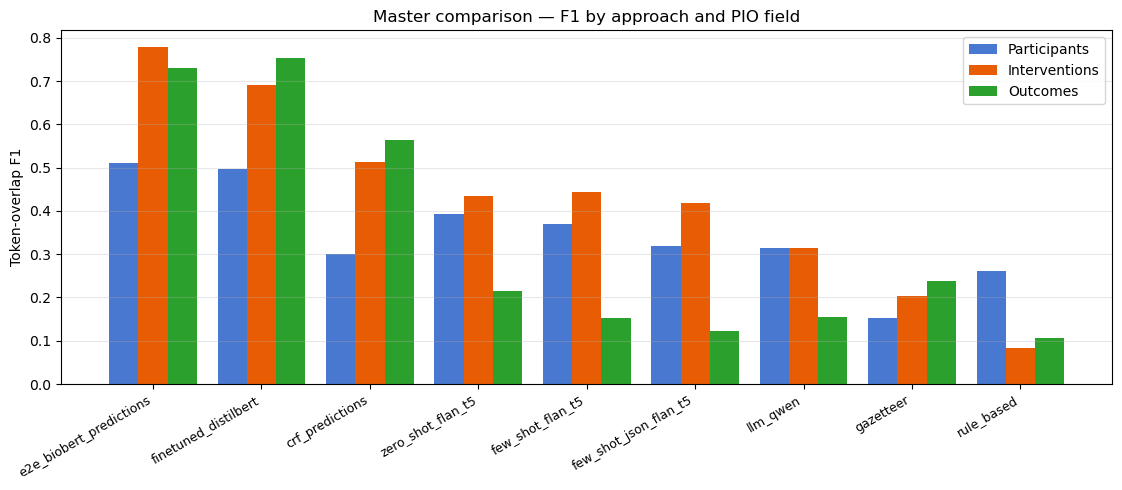
\includegraphics[width=0.95\textwidth]{figures/master_f1_comparison.png}
\caption{Token-overlap F1 by approach and PICO field on the locked
50-doc test set, ordered by macro F1. Approach labels match Table~\ref{tab:master}
(\texttt{e2e\_biobert\_predictions} = E2E BioBERT,
\texttt{finetuned\_distilbert} = DistilBERT,
\texttt{crf\_predictions} = CRF, etc.).}
  \label{fig:master_f1}
\end{figure*}

Three observations stand out. First, fine-tuning dominates: the two
fine-tuned transformers (BioBERT, DistilBERT) score roughly twice the
macro F1 of the best prompted LLM (zero-shot flan-T5, 0.347), confirming
H3 strongly --- with $\sim$4{,}500 training documents available,
fine-tuning is the right choice. Second, H1 holds for fine-tuned LLMs
but only partially for prompted ones: regex and gazetteer (0.150 and
0.198 macro F1) are beaten by every LLM-based approach including
Qwen3-0.6B (0.261), yet the gazetteer beats every prompted LLM on
Outcomes precision (0.572 vs 0.337--0.493) because the
highest-frequency outcome 1-grams (\texttt{score}, \texttt{rate},
\texttt{adverse}) are concentrated near the gold spans. Third, Outcomes
is the hardest field for every approach: even E2E BioBERT loses almost
five points of F1 on Outcomes vs Interventions (0.730 vs 0.778), because
outcomes have varied surface forms (\textit{blood pressure},
\textit{quality of life}, \textit{adverse events}) where interventions
are usually named drugs or procedures that anchor the answer
lexically. We return to this in error analysis.
\paragraph{Statistical caveat on Table~\ref{tab:master}.} With $n\!=\!50$
documents, per-document F1 has substantial variance. The bootstrap
analysis we ran on the flan-T5 prompting variants
(Table~\ref{tab:bootstrap}) shows 95\% CIs typically spanning $\pm 0.05$
F1 at this sample size. Small differences in Table~\ref{tab:master}
should therefore be interpreted carefully: the gap between E2E BioBERT
($0.673$) and DistilBERT ($0.647$) is $0.026$ macro F1, well within
plausible bootstrap uncertainty, and we treat the top-2 ranking as a
tie. Larger gaps e.g. CRF ($0.459$) versus either fine-tuned
transformer, or any fine-tuned model versus any prompted LLM --- are
well outside this margin and we treat them as reliable.

\subsection{Axis B under strict span F1 (secondary metric)}
\label{sec:e2e_vs_dec}

Table~\ref{tab:nb05_nb06} reports the within-notebook comparisons for
axis B, using each notebook's own metric so the comparison is internally
consistent.

\begin{table*}[tbp]
\centering
\small
\begin{tabular}{lccc|ccc|ccc|c}
\toprule
& \multicolumn{3}{c}{\textbf{Participants}} & \multicolumn{3}{c}{\textbf{Interventions}} & \multicolumn{3}{c}{\textbf{Outcomes}} & \\
\cmidrule(lr){2-4}\cmidrule(lr){5-7}\cmidrule(lr){8-10}
\textbf{Approach} & P & R & F1 & P & R & F1 & P & R & F1 & \textbf{Macro F1} \\
\midrule
\multicolumn{11}{l}{\textit{NB06: strict span F1 (BIO sequences)}}\\
CRF                    & .300 & .128 & .180 & .572 & .284 & .379 & .369 & .175 & .238 & .265 \\
E2E BioBERT            & .253 & .262 & .258 & .608 & .583 & \textbf{.595} & .456 & .414 & \textbf{.434} & \textbf{.429} \\
Decomposed BioBERT     & .225 & .252 & .237 & .605 & .366 & .456 & .400 & .376 & .388 & .360 \\
\midrule
\multicolumn{11}{l}{\textit{NB05: token-overlap F1 (extractive QA)}}\\
QA end-to-end          & .833 & .357 & .443 & .321 & .205 & .209 & .312 & .121 & .157 & .270 \\
QA decomposed (2-step) & .696 & .438 & \textbf{.493} & .412 & .342 & .344 & .403 & .330 & \textbf{.335} & \textbf{.391} \\
QA decomposed (3-step) & .658 & .366 & .423 & .314 & .272 & .269 & .406 & .329 & .335 & .342 \\
\bottomrule
\end{tabular}
\caption{Axis~B comparisons. NB06 reports strict span F1 (the standard
NER metric); NB05 reports token-overlap F1 to be consistent with the
master comparison. The two notebooks therefore answer the same question
under different difficulty levels.}
\label{tab:nb05_nb06}
\end{table*}

The interaction of the underlying model with the decomposition is the
most informative result in the project. \textbf{For QA on
RoBERTa-SQuAD2}, decomposing helps a lot: 2-step lifts macro F1 from
0.270 to 0.391 ($+12$ points), driven mainly by Interventions and
Outcomes. The relevance step removes background sentences from which
the QA model otherwise produces low-confidence spurious spans.
\textbf{For BioBERT trained directly on token-level annotations}, the
opposite happens: decomposing drops macro F1 from 0.429 to 0.360
($-7$ points). The TF-IDF + LR classifier filters out around 40\% of
sentences containing entity tokens (recall drops by 0.05--0.21 across
fields while precision is essentially unchanged), and once a sentence
is discarded those tokens cannot be recovered. \textbf{H4 (decomposing
improves precision) therefore holds only when the underlying extractor
is the bottleneck}; when the extractor is already strong, decomposing
is a net loss.

The 3-step QA pipeline (heuristic cleaning) is uniformly worse than
2-step. The ``person word'' filter for Participants is too aggressive:
a span like \textit{``100 elderly Norwegians''} is dropped because
\textit{Norwegian} is not in the keyword list.

\subsection{Statistical reliability of the prompted-LLM comparison}

With 50 evaluation documents, per-document F1 is noisy. We ran a paired
bootstrap (2{,}000 resamples) on the three flan-T5 prompting variants
(NB03). Mean F1 with 95\% confidence intervals is shown in
Table~\ref{tab:bootstrap}. Only three pairwise differences are
significant at $\alpha\!=\!0.05$: zero-shot beats few-shot+JSON on both
Participants and Outcomes, and zero-shot beats few-shot on Outcomes.
The remaining six comparisons are within noise.

\begin{table*}[tbp]
\centering
\small
\begin{tabular}{l c c c c c c}
\toprule
& \multicolumn{2}{c}{\textbf{Participants}} & \multicolumn{2}{c}{\textbf{Interventions}} & \multicolumn{2}{c}{\textbf{Outcomes}} \\
\cmidrule(lr){2-3}\cmidrule(lr){4-5}\cmidrule(lr){6-7}
\textbf{Approach} & F1 & 95\% CI & F1 & 95\% CI & F1 & 95\% CI \\
\midrule
flan-T5 zero-shot     & .360 & [.284, .435] & .385 & [.316, .454] & .198 & [.149, .250] \\
flan-T5 few-shot      & .339 & [.261, .421] & .393 & [.332, .452] & .143 & [.107, .180] \\
flan-T5 few-shot+JSON & .289 & [.214, .369] & .366 & [.300, .431] & .114 & [.078, .154] \\
\midrule
zero-shot $-$ few-shot       & $+$.020 & [$-$.045, $+$.086] & $-$.008 & [$-$.061, $+$.053] & $\boxed{+.054}$ & [$+$.004, $+$.110] \\
zero-shot $-$ few-shot+JSON  & $\boxed{+.070}$ & [$+$.012, $+$.134] & $+$.019 & [$-$.049, $+$.092] & $\boxed{+.084}$ & [$+$.037, $+$.135] \\
few-shot  $-$ few-shot+JSON  & $\boxed{+.050}$ & [$+$.018, $+$.086] & $+$.027 & [$-$.018, $+$.075] & $+$.030 & [$-$.009, $+$.065] \\
\bottomrule
\end{tabular}
\caption{Per-approach F1 with bootstrap 95\% CIs and pairwise
differences (paired bootstrap, 2{,}000 resamples). Boxed values are
significant. Note that Interventions is the field where prompt format
matters \textit{least} --- named drugs anchor the answer regardless.}
\label{tab:bootstrap}
\end{table*}

\subsection{Coverage versus correctness, and the placebo failure mode}

The four prompted LLMs all report 100\% coverage they always emit
\textit{something} --- but their macro recall sits between 0.24 and 0.42
(Figure~\ref{fig:pr}). The clinical cost of this trade-off is concrete:
the gold annotations identify 11 placebo-controlled trials in the
locked set, but the four prompted approaches retrieve only 1, 1, 1
and 4 of them respectively when we run the keyword query
\textit{trials with placebo} against the extracted Interventions
column. Every fine-tuned model and every rule-based approach retrieves
at least 11. The gazetteer wins this query outright because
\texttt{placebo} is a top-50 training-set term a baseline that
costs nothing to build retrieves \textit{more} placebo trials than a
250M-parameter language model. High coverage is not a substitute for
high recall on the surface forms that downstream queries depend on.

\begin{figure}[tbp]
  \centering
  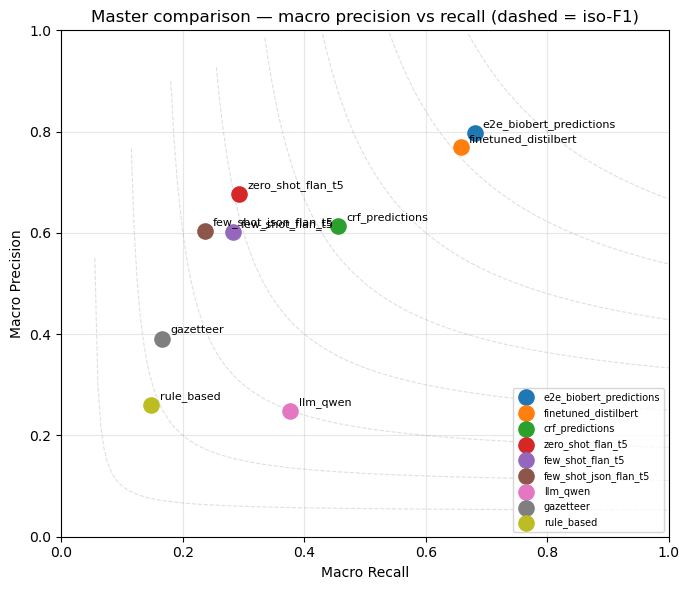
\includegraphics[width=\columnwidth]{figures/master_precision_recall.png}
  \caption{Macro precision vs recall by approach (dashed lines are
  iso-F1 contours). Prompted LLMs cluster on the high-precision,
  low-recall side; fine-tuned models reach both.}
  \label{fig:pr}
\end{figure}

\subsection{Error analysis}
\label{sec:errors}

We grouped per-document errors by failure mode using NB03's analysis
cells (false positives, false negatives, empty outputs) plus inspection
of the worst 10 documents per approach. Five patterns emerged.

\paragraph{Few-shot priming bias (prompted LLMs).} The few-shot block
contains a worked example that mentions ``Rhinocort Study Group''. For
doc 10070173, the few-shot extractor copies this string verbatim into
the Participants field of the new abstract it does not appear in
the test abstract at all. Few-shot examples therefore function as soft
priors that the model is reluctant to discard. This explains why
few-shot loses to zero-shot on Outcomes (where the example shapes the
lexical distribution most strongly): the example floods the output
with terms that don't belong to the new trial.

\paragraph{JSON placeholder leakage (NB03 few-shot+JSON).} The literal
string ``\texttt{not specified}'' appears in 15 of 50 outcome
predictions, by far the most common false-positive token in the JSON
condition. The few-shot block contains the fallback
\texttt{"answer": "not specified"} for one example with no outcome; the
model copies it verbatim when uncertain rather than emitting the empty
string. The JSON constraint is itself fine; the failure is providing a
non-empty placeholder in the example.

\paragraph{Length sensitivity (flan-T5).} F1 has a clear negative slope
against abstract length for Participants (regression coefficient
$-2 \times 10^{-3}$ per token), is approximately flat for Interventions,
and trends mildly \textit{positive} for Outcomes. The plausible reason
is that flan-T5-base has a 512-token input limit; once the abstract
plus three-shot prompt exceeds that limit, the truncation discards the
tail of the abstract. Participants are normally introduced in the first
1--2 sentences, so they are robust to truncation only on short
abstracts. Outcomes appear throughout, so longer abstracts give the
model more correct tokens to land on even after truncation.

\paragraph{Decomposed BioBERT under-recall (NB06).} Filter recall on the
sentence-classification step is 70--85\% per field, but participants
sometimes appear in single-sentence abstracts where the methods clause
is fused with the patient description (``\textit{Eighty-six male
volunteers received a single dose of \dots}''). The TF-IDF classifier
confuses this with a methods sentence and discards it. Including
sentence position as a feature would likely recover most of the lost 
participants recall.

\paragraph{Outcomes are systematically under-extracted across all
approaches.} Most-missed gold tokens for E2E BioBERT include
\textit{long-term}, \textit{quality-of-life}, \textit{economic} and
\textit{ergometric} compound modifiers that the BIO scheme treats
as start-of-span on a low-frequency token. Per-field model capacity is
not the bottleneck; the annotation scheme is.

\paragraph{Compute cost.} Approaches differ by four orders of magnitude
in training time. The CRF baseline trains in under 60 seconds on CPU.
Fine-tuned DistilBERT trains in roughly 200--600 seconds per field on a
Colab T4 GPU, under 30 minutes total across the three fields. End-to-end
BioBERT trains in roughly 90 minutes on the same GPU (4 epochs head-only
at $5\!\times\!10^{-5}$, then 2 epochs full fine-tune at
$2\!\times\!10^{-5}$). The decomposed BioBERT pipeline is the most
expensive at $\sim$13 hours of CPU-equivalent compute due to per-field
training. flan-T5 inference takes 15--25 minutes for 50 documents
across three prompting variants on CPU. Whether the $0.21$ macro F1 gap
from CRF ($0.459$) to E2E BioBERT ($0.673$) is worth a $\sim$90$\times$
compute increase depends on corpus scale: for a one-off review of
$<$1{,}000 abstracts, CRF is the practical choice; for an
evidence-synthesis pipeline running over PubMed, BioBERT amortises over
throughput.

\subsection{The deliverable: a structured PICO table}

The final output of the system is the structured table that the brief
asks for. NB07 emits \texttt{extracted\_pico\_best.csv} (best approach,
50 rows, $\sim$8 columns) and \texttt{extracted\_pico\_all.csv} (long
format with every approach side-by-side). Table~\ref{tab:pico_sample}
shows two example rows from the best approach (E2E BioBERT) for
qualitative inspection.

Three observations on the deliverable. First, multi-span fields are
preserved by $\vert$-separated lists, so a downstream query for
``trials in children'' matches PMID 10390665 even though
\texttt{children} is one of three Population spans. Second, the
extraction occasionally surfaces noisy inclusion criteria as
Participants (e.g. PMID 10589810 reports just \texttt{40 $\vert$ 20},
losing the underlying cohort description) a query-time filter on
span length would catch this. Third, comparators remain conflated with
interventions (\textit{granisetron $\vert$ perphenazine} for PMID
10390665 mixes the active drug and its comparator), reflecting the
EBM-NLP annotation scheme rather than a model failure
(\S\ref{sec:limitations}).

\begin{table*}[!t]
\centering
\small
\begin{tabularx}{\textwidth}{l X X X}
\toprule
\textbf{PMID} & \textbf{Participants} & \textbf{Interventions} & \textbf{Outcomes} \\
\midrule
10390665 & children $\vert$ 90 paediatric $\vert$ aged 4--10 years
         & granisetron $\vert$ perphenazine
         & Anti-emetic efficacy $\vert$ post-operative $\vert$ complete response \\
10589810 & 40 $\vert$ 20
         & root instrumentation $\vert$ conventional steel $\vert$ plastic curettes
         & bleeding on probing (BOP) $\vert$ probing pocket depth (PPD) \\
\bottomrule
\end{tabularx}
\caption{Two sample rows from \texttt{extracted\_pico\_best.csv}
(E2E BioBERT). The Population is sometimes split into multiple spans
(``children'' + sample size + age) which the table preserves with
$\vert$ separators; downstream queries can match against any.}
\label{tab:pico_sample}
\end{table*}


\section{Conclusions}

Table~\ref{tab:hyp_verdicts} summarises the verdict on each of the five
hypotheses from \S\ref{sec:hypotheses} against the experimental data in
\S\ref{sec:results}.

\begin{table}[H]
\centering
\small
\begin{tabular}{cp{2.5cm}p{3.7cm}}
\toprule
\textbf{H} & \textbf{Claim} & \textbf{Verdict} \\
\midrule
H1 & LLM $>$ rule-based      & \checkmark{} Confirmed (0.15 macro F1 gap) \\
H2 & Few-shot $>$ zero-shot  & $\times${} Rejected on Outcomes ($p\!<\!0.05$); n.s.\ elsewhere \\
H3 & Fine-tuned $>$ prompted & \checkmark{} Confirmed strongly (1.94$\times$ F1) \\
H4 & Decompose $\to$ better precision & $\circ${} Conditional: helps QA, hurts BioBERT \\
H5 & BioBERT $>$ DistilBERT  & $\circ${} Tie within bootstrap CI ($\pm$0.05) \\
\bottomrule
\end{tabular}
\caption{Hypothesis verdicts. \checkmark{} confirmed, $\times${}
rejected, $\circ${} partial or conditional.}
\label{tab:hyp_verdicts}
\end{table}

\paragraph{What worked, and what we recommend.} For a deployed PICO
extraction system over PubMed-scale corpora, we recommend end-to-end
BioBERT with the two-phase fine-tuning recipe (head-only at
$5\!\times\!10^{-5}$, then full fine-tune at $2\!\times\!10^{-5}$); for
a one-off review of fewer than 1{,}000 abstracts, CRF delivers roughly
70\% of the F1 at 1\% of the compute and is the better practical choice.
Fine-tuning a domain-pretrained transformer on the EBM-NLP training
split is the right approach for this task at this data scale: end-to-end
BioBERT achieves a macro token-overlap F1 of 0.673, clearly above every
other approach we tested.

\paragraph{What did not work as expected.} Three of our five hypotheses
were challenged by the experiments. Zero-shot beats few-shot for
flan-T5 on Outcomes ($+$0.054 F1, significant) because few-shot
examples prime the model with study-specific phrases that leak into
unrelated abstracts. Decomposing extraction helps the QA model
($+$0.12 macro F1) but hurts BioBERT ($-$0.07 strict span F1), because
the TF-IDF relevance filter is the bottleneck of the pipeline rather
than the extractor. Adding a JSON output constraint hurts every field,
mainly because the literal placeholder string in the few-shot example
leaks into 30\% of empty cases.

\paragraph{Open challenges.} Four challenges remain. First, comparator
extraction: EBM-NLP folds the comparator into the Interventions field
by design, and although NB05 implements a keyword-based post-processing
step (\textit{vs}, \textit{compared to}, \textit{control},
\textit{placebo}) that splits intervention spans, we could not evaluate
it quantitatively against any reference annotation; building a
re-annotation of EBM-NLP with a separate Comparator field is a clear
next step. Second, the coverage--correctness gap: a 100\% coverage
rate masks the fact that prompted LLMs retrieve 1 out of 11
placebo-controlled trials on a downstream keyword query, so any
deployed system should report a recall-at-query metric in addition to
F1 because the latter does not penalise systematic absence of common
surface forms. Third, length sensitivity: the 512-token input limit of
flan-T5-base imposes a hard ceiling on Participants extraction quality
for long abstracts, and either a model with a longer context window
(e.g.\ Long-T5 \citep{guo2022longt5}) or a sliding-window inference
strategy would address this without changing the prompting axis.
Fourth, annotation cost: the compound-modifier failure mode in the
error analysis suggests that EBM-NLP's BIO scheme under-represents
multi-word outcome terms; future work should re-annotate at the chunk
level for fairer evaluation of long outcome spans.

\label{sec:limitations}
\paragraph{Limitations of this study.} The locked evaluation set is 50
documents chosen so that every notebook can be re-run on a single
T4 GPU  and bootstrap CIs at this size are typically $\pm 0.05$ F1.
Differences smaller than this should be treated as noise. The QA
predictions in NB05 were generated against a pre-locked document set
and therefore appear with zero coverage on the master comparison; we
report them in Table~\ref{tab:nb05_nb06} so the
decomposed-vs-end-to-end axis remains visible.


\bibliographystyle{acl_natbib}

\begin{thebibliography}{99}

\bibitem[Chung et al.(2022)]{chung2022flan}
Hyung Won Chung, Le Hou, Shayne Longpre, Barret Zoph, Yi Tay,
William Fedus, Eric Li, Xuezhi Wang, Mostafa Dehghani, Siddhartha
Brahma, et~al.
\newblock 2022.
\newblock Scaling instruction-finetuned language models.
\newblock \emph{arXiv preprint arXiv:2210.11416}.

\bibitem[Deka and Pal(2022)]{deka2022pubmed}
Pritam Deka and Ankur Pal.
\newblock 2022.
\newblock S-PubMedBert-MS-MARCO.
\newblock HuggingFace model card,
\newblock \url{https://huggingface.co/pritamdeka/S-PubMedBert-MS-MARCO}.

\bibitem[Devlin et al.(2019)]{devlin2019bert}
Jacob Devlin, Ming-Wei Chang, Kenton Lee, and Kristina Toutanova.
\newblock 2019.
\newblock BERT: Pre-training of deep bidirectional transformers for
language understanding.
\newblock In \emph{Proceedings of NAACL-HLT}, pages 4171--4186.

\bibitem[Guo et al.(2022)]{guo2022longt5}
Mandy Guo, Joshua Ainslie, David Uthus, Santiago Onta\~n\'on,
Jianmo Ni, Yun-Hsuan Sung, and Yinfei Yang.
\newblock 2022.
\newblock LongT5: Efficient text-to-text transformer for long sequences.
\newblock In \emph{Findings of NAACL}.

\bibitem[Higgins et al.(2019)]{higgins2019cochrane}
Julian P.~T. Higgins, James Thomas, Jacqueline Chandler, Miranda
Cumpston, Tianjing Li, Matthew~J. Page, and Vivian~A. Welch, editors.
\newblock 2019.
\newblock \emph{Cochrane Handbook for Systematic Reviews of
Interventions (version 6)}.
\newblock John Wiley \& Sons.

\bibitem[Lafferty et al.(2001)]{lafferty2001crf}
John Lafferty, Andrew McCallum, and Fernando C.~N. Pereira.
\newblock 2001.
\newblock Conditional random fields: probabilistic models for
segmenting and labeling sequence data.
\newblock In \emph{Proceedings of ICML}, pages 282--289.

\bibitem[Lee et al.(2020)]{lee2020biobert}
Jinhyuk Lee, Wonjin Yoon, Sungdong Kim, Donghyeon Kim, Sunkyu Kim,
Chan Ho So, and Jaewoo Kang.
\newblock 2020.
\newblock BioBERT: a pre-trained biomedical language representation
model for biomedical text mining.
\newblock \emph{Bioinformatics}, 36(4):1234--1240.

\bibitem[Liu et al.(2019)]{liu2019roberta}
Yinhan Liu, Myle Ott, Naman Goyal, Jingfei Du, Mandar Joshi, Danqi
Chen, Omer Levy, Mike Lewis, Luke Zettlemoyer, and Veselin Stoyanov.
\newblock 2019.
\newblock RoBERTa: A robustly optimized BERT pretraining approach.
\newblock \emph{arXiv preprint arXiv:1907.11692}.

\bibitem[Nye et al.(2018)]{nye2018ebmnlp}
Benjamin Nye, Junyi Jessy Li, Roma Patel, Yinfei Yang, Iain
Marshall, Ani Nenkova, and Byron Wallace.
\newblock 2018.
\newblock A corpus with multi-level annotations of patients,
interventions and outcomes to support language processing for medical
literature.
\newblock In \emph{Proceedings of ACL}, pages 197--207.

\bibitem[Qwen Team(2024)]{qwen2024}
Qwen Team.
\newblock 2024.
\newblock Qwen3 technical report.
\newblock Alibaba Cloud,
\newblock \url{https://qwenlm.github.io/}.

\bibitem[Reimers and Gurevych(2019)]{reimers2019sentencebert}
Nils Reimers and Iryna Gurevych.
\newblock 2019.
\newblock Sentence-BERT: Sentence embeddings using Siamese
BERT-networks.
\newblock In \emph{Proceedings of EMNLP-IJCNLP}, pages 3982--3992.

\bibitem[Sanh et al.(2019)]{sanh2019distilbert}
Victor Sanh, Lysandre Debut, Julien Chaumond, and Thomas Wolf.
\newblock 2019.
\newblock DistilBERT, a distilled version of BERT: smaller, faster,
cheaper and lighter.
\newblock In \emph{NeurIPS Workshop on Energy Efficient Machine Learning
and Cognitive Computing}.

\end{thebibliography}

\end{document}